\section*{Magnetometer Mapping}
    With a moving box enclosing the magnetometer at any time, this method allows us to recover the coverage of the area by the magnetometer. Thus we have a way to know precisely the coverage of the mapping during the mission, which depends on the uncertainty on the position of the magnetometer and on the maximum distance of each point of the field to be measured. An example of the covered area of a magnetometer on a field is presented by the \textsc{Figure}~\ref{fig:thickset_trajectory}.

    \begin{figure}[!htb]
        \centering
        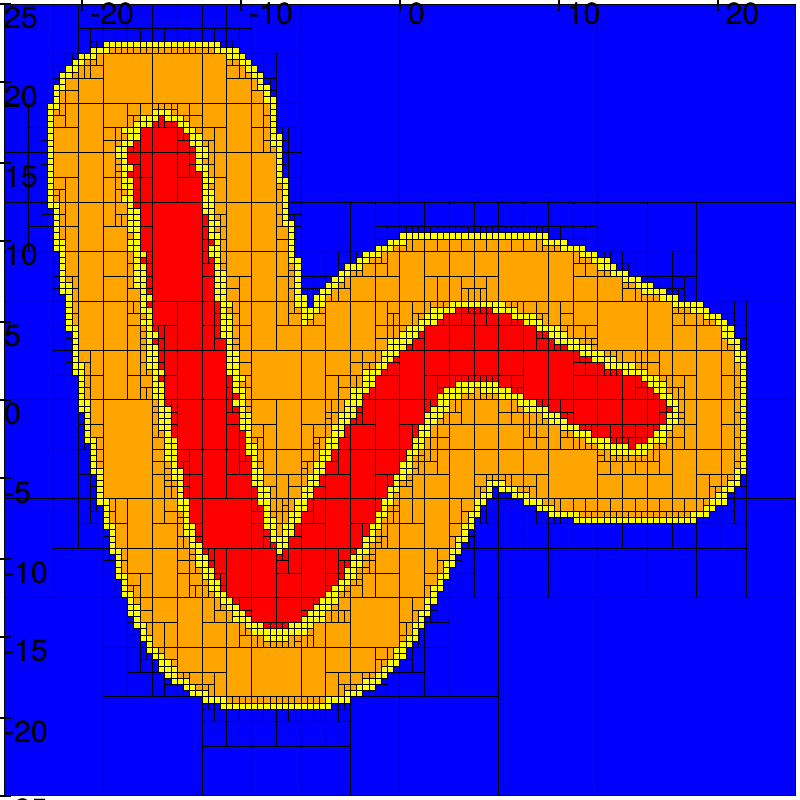
\includegraphics[width=0.4\textwidth]{imgs/thickset_fine.png}
        \caption{\label{fig:thickset_trajectory} Coverage of the map by the magnetometer using Thicksets}
    \end{figure}
    
    